\documentclass[12pt]{article}
\usepackage[letterpaper, margin=1in]{geometry}
\usepackage{graphicx}
\usepackage{subcaption}
\graphicspath{{./Figures/}}
\usepackage{hyperref}
\usepackage{parskip}
\usepackage{amsmath}
\usepackage{amssymb}
\usepackage{mathrsfs}
\usepackage{enumitem}
\allowdisplaybreaks

\title{ELECENG 3CL4 Lab 3 Pre-lab}
\author{
    Aaron Pinto \\
    pintoa9 \\
    L02
    \and
    Raeed Hassan \\
    hassam41 \\
    L02
}

\begin{document}

\maketitle
\clearpage

\section{Proportional Control of DC Motor}
\textbf{Pre-Lab Question 1}
The closed loop transfer function $T(s)$ is:
\begin{equation*}
\begin{aligned}[b]
    T(s) &= \frac{G(s)G_c(s)}{1 + G(s)G_c(s)} \\
    &= \frac{k_pG(s)}{1 + k_pG(s)}
\end{aligned}
\end{equation*}
We find the characteristic equation of the closed loop transfer function $T(s)$ below: 
\begin{equation*}
\begin{aligned}[b]
    0 &= 1 + k_pG(s) \\
    0 &= 1 + \frac{k_pA}{s(s\tau_m + 1)} \\
    0 &= 1 + \frac{k_pA}{s^2\tau_m + s} \\
    -1 &= \frac{k_pA}{s^2\tau_m + s} \\
    -s^2\tau_m - s &= k_pA \\
    0 &= s^2\tau_m + s + k_pA
\end{aligned}
\end{equation*}
The closed-loop poles of the system is found by determining the poles of the characteristic equation, which is done in Equation~\ref{eq:1}.  
\begin{equation} \label{eq:1}
\begin{aligned}[b]
    p_{1,2} &= \frac{-b \pm \sqrt{b^2 - 4ac}}{2a} \\
    a &= \tau_m, \ b = 1, \ c = k_pA \\
    &= \frac{-1 \pm \sqrt{1 - 4\tau_m k_p A}}{2\tau_m} \\
    p_{1,2} &= -\frac{1}{2\tau_m} \pm \frac{1}{2\tau_m}\sqrt{1 - 4k_p A \tau_m}
\end{aligned}
\end{equation}

\textbf{Pre-Lab Question 2}
\begin{figure}
    \centering
    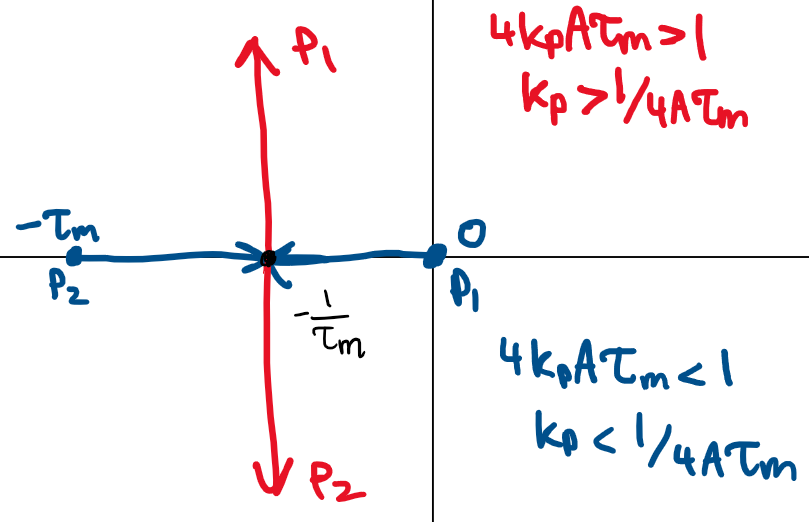
\includegraphics[width=\textwidth]{q2}
    \caption{\label{fig:2}q2}
\end{figure}

\textbf{Pre-Lab Question 3}
\begin{equation*}
\begin{aligned}[b]
    T(s) &= \frac{k_pG(s)}{1 + k_pG(s)} \\
    &= \frac{\frac{k_pA}{s^2\tau_m + s}}{1 + \frac{k_pA}{s^2\tau_m + s}} \\
    &= \frac{k_pA}{s^2\tau_m + s + k_pA} \\
    &= \frac{\frac{k_pA}{\tau_m}}{s^2 + \frac{s}{\tau_m} + \frac{k_pA}{\tau_m}} \\
    F_2(s) &= \frac{\omega_n^2}{s^2 + 2\zeta\omega_ns + \omega_n^2} \\
    \omega_n^2 &= \frac{k_pA}{\tau_m} \\
    \omega_n &= \sqrt{\frac{k_pA}{\tau_m}} \\
    2\zeta\omega_ns &= \frac{s}{\tau_m} \\
    \zeta\omega_n &= \frac{1}{2\tau_m} \\
    \zeta &= \frac{1}{2\tau_m\omega_n} \\
    \zeta &= \frac{1}{2\tau_m\sqrt{\frac{k_pA}{\tau_m}}} \\
    \zeta &= \frac{1}{2\sqrt{k_pA\tau_m}}
\end{aligned}
\end{equation*}

\textbf{Pre-Lab Question 4}
\begin{equation*}
\begin{aligned}[b]
    \zeta &= \frac{1}{2\sqrt{k_pA\tau_m}} \\
    &= \frac{1}{2\sqrt{\frac{A\tau_m}{4A\tau_m}}} \\
    &= \frac{1}{2\sqrt{\frac{1}{4}}} \\
    &= \frac{1}{2(0.5)}
    \zeta &= 1
\end{aligned}
\end{equation*}
c'est critically damped

\textbf{Pre-Lab Question 5}
\begin{equation*}
\begin{aligned}[b]
    p_{1,2} &= -\frac{1}{2\tau_m} \pm \frac{1}{2\tau_m}\sqrt{1 - 4k_p A \tau_m} \\
    &= \frac{1}{2\tau_m} \left( -1 \pm \sqrt{1 - 4k_p A \tau_m} \right)
\end{aligned}
\end{equation*}

\section{Trade-offs in Proportional Control of a Servomotor: Theoretical Insight}
\textbf{Pre-Lab Question 6}
\begin{align*}
    T_s &\approx \frac{4}{\zeta\omega_n} \\
    &\approx \frac{4}{\frac{\omega_n}{2\omega_n\tau_m}} \\
    &\approx \frac{4}{\frac{1}{2\tau_m}} \\
    &\approx 8\tau_m \\
    P.O. &= 100\exp\left(-\frac{\pi\zeta}{\sqrt{1-\zeta^2}}\right) \\
    &= 100\exp\left(-\frac{\frac{\pi}{2\omega_n\tau_m}}{\sqrt{1-\left(\frac{1}{2\omega_n\tau_m}\right)^2}}\right) \\
    &= 100\exp\left(-\frac{\frac{\pi}{2\omega_n\tau_m}}{\sqrt{1-\frac{1}{4\omega_n^2\tau_m^2}}}\right) \\
    &= 100\exp\left(-\frac{\pi}{2\omega_n\tau_m\sqrt{1-\frac{1}{4\omega_n^2\tau_m^2}}}\right) \\
    % &= 100\exp\left(-\frac{\pi}{2\omega_n\tau_m\sqrt{\frac{4\omega_n^2\tau_m^2}{4\omega_n^2\tau_m^2}-\frac{1}{4\omega_n^2\tau_m^2}}}\right) \\
    &= 100\exp\left(-\frac{\pi}{2\omega_n\tau_m\sqrt{\frac{4\omega_n^2\tau_m^2 - 1}{4\omega_n^2\tau_m^2}}}\right) \\
    &= 100\exp\left(-\frac{\pi}{2\omega_n\tau_m\frac{\sqrt{4\omega_n^2\tau_m^2 - 1}}{\sqrt{4\omega_n^2\tau_m^2}}}\right) \\
    &= 100\exp\left(-\frac{\pi}{\sqrt{4\omega_n^2\tau_m^2 - 1}}\right) \\
    &= 100\exp\left(-\frac{\pi}{\sqrt{4\frac{k_pA}{\tau_m}\tau_m^2 - 1}}\right) \\
    &= 100\exp\left(-\frac{\pi}{\sqrt{4k_pA\tau_m - 1}}\right) \\
    T_{r1} &\approx \frac{2.16\zeta + 0.6}{\omega_n} \\
    &\approx \frac{\frac{2.16}{2\omega_n\tau_m} + 0.6}{\omega_n} \\
    &\approx \frac{\frac{2.16 + 1.2\omega_n\tau_m}{2\omega_n\tau_m}}{\omega_n} \\
    &\approx \frac{2.16 + 1.2\omega_n\tau_m}{2\omega_n^2\tau_m} \\
    &\approx \frac{2.16 + 1.2\sqrt{\frac{k_pA}{\tau_m}}\tau_m}{2\frac{k_pA}{\tau_m}\tau_m} \\
    &\approx \frac{2.16 + 1.2\sqrt{k_pA\tau_m}}{2k_pA} \\
\end{align*}

\textbf{Pre-Lab Question 7}
$T_s$ does not change with $k_p$. P.O. increases as $k_p$ increases and it approaches a horizontal asymptote of 100\%. $T_{r1}$ decreases as $k_p$ decreases and approaches the horizontal asymptote of 0.

\textbf{Pre-Lab Question 8}
The 2\% settling time will not change no matter what we do for $k_p$.

\textbf{Pre-Lab Question 9}

\textbf{Pre-Lab Question 10}

\textbf{Pre-Lab Question 11}


\setcounter{section}{5}
\section{Proportional Controller with Velocity Feedback}
\textbf{Pre-Lab Question 12}
If we use block diagram transforms we can transform the block diagram to Figure(ref figure here).
\begin{figure}
    \centering
    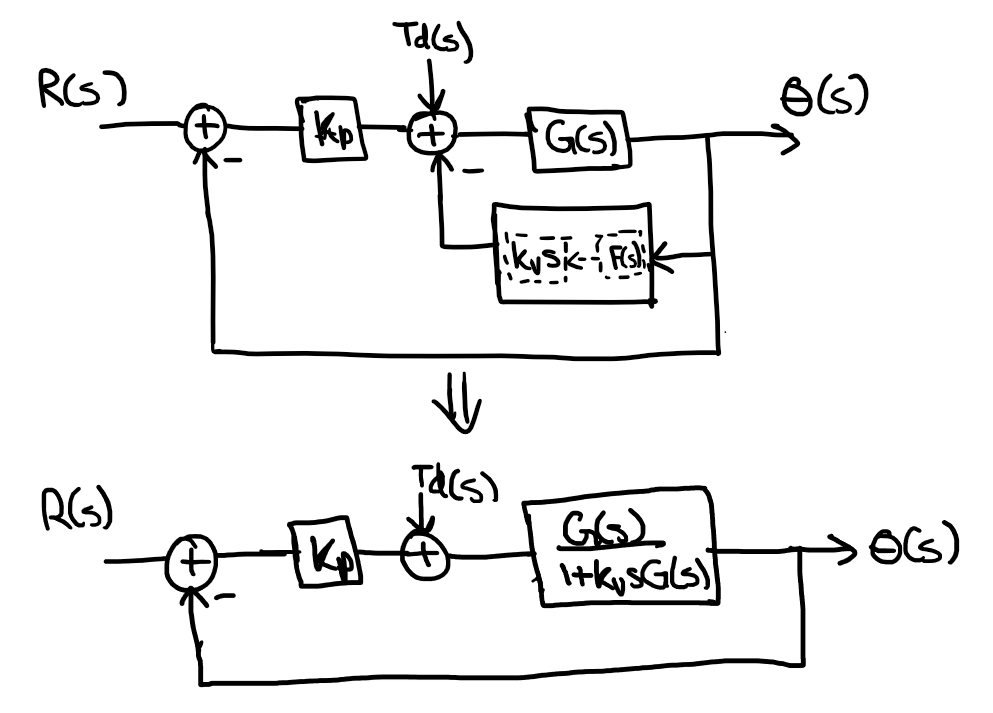
\includegraphics[width=\textwidth]{q12}
    \caption{\label{fig:12}q12}
\end{figure}
From the block diagram, we can see that the total output response when $F(s) \approx 1$ can be written as:
\begin{equation}
\begin{aligned}[b]
    \Theta(s) &= \frac{k_pG(s)}{1 + k_vsG(s) + k_pG(s)}R(s) + \frac{G(s)}{1 + k_vsG(s) + k_pG(s)}T_d(s) \\
    &= \frac{\frac{k_pA}{s(s\tau_m + 1)}}{1 + s\frac{k_vA}{s(s\tau_m + 1)} + \frac{k_pA}{s(s\tau_m + 1)}}R(s) + \frac{\frac{A}{s(s\tau_m + 1)}}{1 + s\frac{k_vA}{s(s\tau_m + 1)} + \frac{k_pA}{s(s\tau_m + 1)}}T_d(s) \\
    &= \frac{k_pA}{s(s\tau_m + 1) + k_vAs + kpA}R(s) + \frac{A}{s(s\tau_m + 1) + k_vAs + kpA}T_d(s) \\
    &= \frac{\frac{k_pA}{\tau_m}}{s^2 + \frac{1+k_vA}{\tau_m}s + \frac{k_pA}{\tau_m}}R(s) + \frac{\frac{A}{\tau_m}}{s^2 + \frac{1+k_vA}{\tau_m}s + \frac{k_pA}{\tau_m}}T_d(s)
\end{aligned}
\end{equation} 

\textbf{Pre-Lab Question 13}
\begin{equation}
\begin{aligned}[b]
    e_{ss} &= \underset{s \rightarrow 0}{\text{lim}}s\frac{A}{s(s\tau_m+1) + k_vAs + k_pA}T_d(s) \\
    &= \underset{s \rightarrow 0}{\text{lim}}s\frac{A}{s(s\tau_m+1) + k_vAs + k_pA}\frac{\tau_d}{s} \\
    &= \underset{s \rightarrow 0}{\text{lim}}\frac{A\tau_d}{s(s\tau_m+1) + k_vAs + k_pA} \\
    &= \frac{A\tau_d}{k_pA + \text{lim}_{s \rightarrow 0} s(s\tau_m+1) + k_vAs} \\
    &= \frac{A\tau_d}{k_pA} \\
    &= \frac{\tau_d}{k_p}
\end{aligned}
\end{equation} 

\textbf{Pre-Lab Question 14}
The closed-loop transfer function can be written as:
\begin{equation*}
\begin{aligned}[b]
    T(s) &= \frac{k_pG(s)}{1 + k_vsG(s) + k_pG(s)} \\
    &= \frac{\frac{k_pA}{s(s\tau_m + 1)}}{1 + \frac{k_vA}{s(s\tau_m + 1)}s + \frac{k_pA}{s(s\tau_m + 1)}} \\
    &= \frac{k_pA}{s^2\tau_m + (1 + k_vA)s + k_pA} \\
    &= \frac{\frac{k_pA}{\tau_m}}{s^2 + \frac{1 + k_vA}{\tau_m}s + \frac{k_pA}{\tau_m}} 
\end{aligned}
\end{equation*}
We can find $\zeta$ by writing the closed-loop transfer function in the form of a standard second-order system.
\begin{equation*}
\begin{aligned}[b]
    F_2(s) &= \frac{\omega_n^2}{s^2 + 2\zeta\omega_ns + \omega_n^2} \\
    \omega_n^2 = \frac{k_pA}{\tau_m} \\
    \omega_n &= \sqrt{\frac{k_pA}{\tau_m}} \\
    2\zeta\omega_ns &= \frac{1+k_vA}{\tau_m}s \\
    \zeta\omega_n &= \frac{1+k_vA}{2\tau_m} \\
    \zeta &= \frac{1+k_vvA}{2\tau_m\omega_n} \\
    \zeta &= \frac{1+k_vA}{2\tau_m\sqrt{\frac{k_pA}{\tau_m}}} \\
    \zeta &= \frac{1+k_vA}{2\sqrt{k_pA\tau_m}}
\end{aligned}
\end{equation*}

\textbf{Pre-Lab Question 15}
Increasing $k_p$ will decrease $\zeta$, which will lead to a decrease in the rise time and an increase in the maximum overshoot, while decreasing $k_p$ will increase the rise time and decrease the maximum overshoot. Increasing $k_v$ will increase $\zeta$, which will lead to an increase in the rise time and a decrease in the maximum overshoot, while decreasing $k_v$ will decrease the rise time and increase the maximum overshoot. The steady-state error to a constant disturbance is inversely proportional to $k_p$. % talk about settling time

\end{document}